\chapter{Zusammenfassung \& Ausblick}
Die Ergebnisse in Tabelle \ref{tab:Auswertung} geben eine gute Übersicht zum Vergleich mit weiteren Topologien, durch die Gewichtung und Normierung lassen sich weitere Angaben ergänzen. Der \gls{IAF} schneidet in der Gesamtbewertung um etwa 0,2 Punkte besser ab, dies liegt hauptsächlich an der optimierten Platzierung der Drossel. Jedoch liegt in dieser Zusammenfassung auch der Nachteil der Schaltung im Falle von Phasenverschiebung. Daher kann diese Topologie nach aktuellen Erkenntnissen nicht für diesen Anwendungsfall empfohlen werden.\\ 


Wie in Kapitel \ref{sec:Grundlagen} erwähnt, sind die Halbleiter Modelle ein essenzieller Teil, daher sollen diese optimiert und in die Simulation zurück geführt werden. Die für diese Schaltung ausgewählten Halbleiter können dazu beschafft und im Prüfstand vermessen werden. Der Messaufbau dazu ist in Abb. \ref{fig:dpt} dargestellt, er beinhaltet die Schaltzelle mit Mess- und Versorgungsgeräten sowie einer Sicherheitssteuerung. Die Messwerterfassung wird über ein Oszilloskop umgesetzt, welches die automatisierten Messpunkte erfasst und speichert.  Anhand dieser Messdaten kann das Modell validiert sowie ergänzt und die Simulationsergebnisse somit optimiert werden. \\

 
\begin{figure}
	\centering
	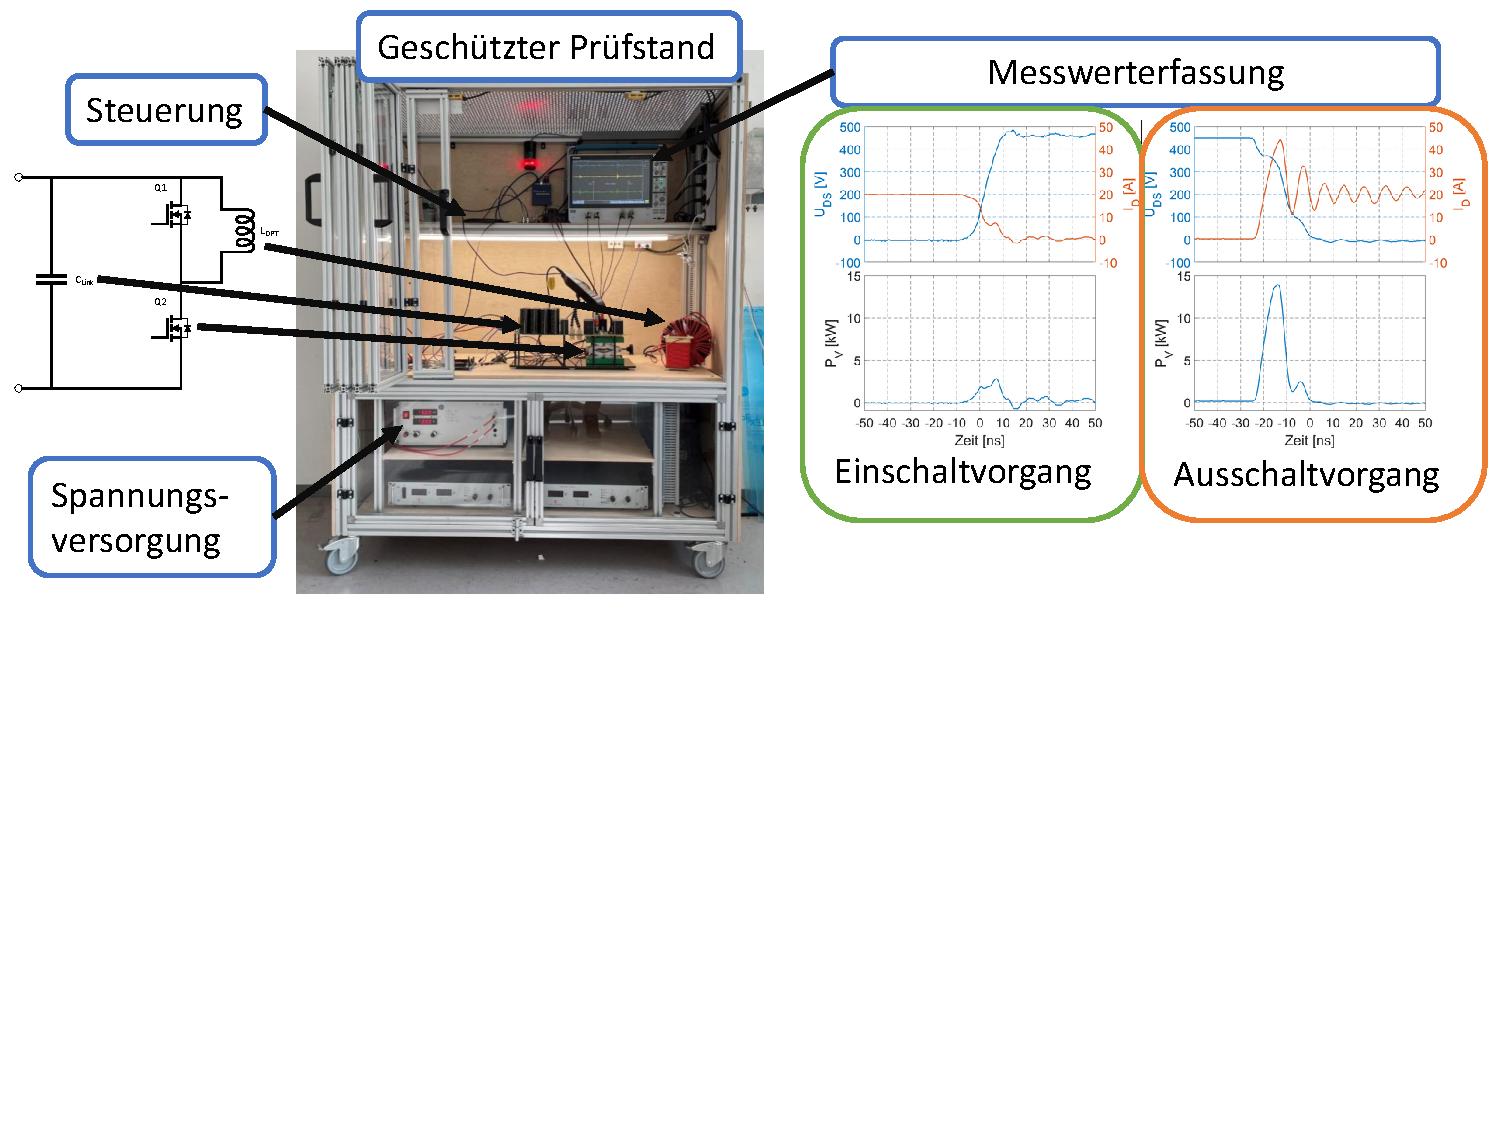
\includegraphics[width=0.9\linewidth]{content/Grafiken/DPT}
	\caption[Doppelpulstestprüfstand]{Doppelpulstestprüfstand}
	\label{fig:dpt}
\end{figure}

Für den Aufbau eines Demonstrators der finalen Topologie, kann die Auslegung der Halbleiter und Drosseln verwendet werden. Die Regelungen können als Grundlage genutzt werden, müssen aber um Sicherheitsfunktionen ergänzt und insbesondere die Stabilität im Gesamtsystem muss sichergestellt werden. Außerdem erfordert die Implementierung auf Hardwarecontrollern weitere Optimierungen. Die Schaltungen können außerdem durch Parallelbetrieb mit Interleaving am Ausgang, oder bei entkoppelter Versorgung als Ausgangsseitige Reihenschaltung Betrieben werden, um eine höhere Ausgangsspannung zu erzielen.  